\documentclass[12pt,a4paper]{article}

\usepackage{amsmath, amsthm, amssymb, amsbsy, amsfonts}
\usepackage[plainpages=false,pdfpagelabels]{hyperref}
\hypersetup{
    colorlinks,
    citecolor=black,
    filecolor=black,
    linkcolor=black,
    urlcolor=blue
}
\usepackage{verbatim}
\usepackage{enumitem}
\usepackage[utf8x]{inputenc}

% Redefine the \vec command to use bold font instead of an arrow
\renewcommand\vec[1]{\mathbf{#1}}

%\def\nl{\hfill\break\null}
\oddsidemargin=0.3cm
\topmargin=-1cm
\textwidth=15cm
\textheight=23cm
\parindent=0cm
\parskip=1mm


\usepackage{graphicx}
\DeclareMathOperator*{\argmin}{argmin}

\newenvironment{enumialpha}{\begin{enumerate}
  \def\theenumi{\alph{enumi}}
  \def\labelenumi{(\theenumi)}}{\end{enumerate}}

\newenvironment{enumiiroman}{\begin{enumerate}
  \def\theenumii{\roman{enumii}}
  \def\labelenumii{(\theenumii)}}{\end{enumerate}}


\begin{document}

\begin{tabular*}{15cm}{@{}l@{\extracolsep{\fill}}r}
  Albert-Ludwigs-Universit\"at Freiburg, Institut f\"ur Informatik \\
PD Dr. Cyrill Stachniss \\  Lecture: Robot Mapping \\
  Winter term 2013 
\end{tabular*}

\bigskip


\begin{center}
{\bf \Large Sheet 4}

{\large Topic: Extended Kalman Filter SLAM}

Submission deadline: Nov.~18\\
Submit to: \texttt{robotmappingtutors@informatik.uni-freiburg.de}
\end{center}

\subsubsection*{Exercise: Implement an EKF SLAM System}

Implement an extended Kalman filter SLAM~(EKF SLAM) system.  To support
this task, we provide a small Octave framework (see course website).
The framework contains the following folders:

\begin{description}
\item [data]  contains files representing the world definition and
    sensor readings.
\item [octave]  contains the EKF SLAM framework with
    stubs  to complete.
\item [plots] this folder is used to store images.
\end{description}

The below mentioned tasks should be implemented inside the framework
in the directory \texttt{octave} by completing the stubs.

After implementing the missing parts, you can run the EKF SLAM system.
To do that, change into the directory \texttt{octave} and launch
\emph{Octave}. Type \texttt{ekf\_slam} to start the main loop (this may
take some time). The program plots the current belief of the robot (pose
and landmarks) in the directory \texttt{plots}.
Figure~\ref{fig:ekfStates} depicts some example images of the state of
the EKF. You can use the images for debugging and to generate an
animation. For example, you can use \emph{ffmpeg} from inside the
\texttt{plots} directory as follows:
\begin{verbatim}
ffmpeg -r 10 -b 500000 -i ekf_%03d.png ekf_slam.mp4
\end{verbatim}

\begin{enumialpha}
    \item
      Implement the prediction step of the EKF SLAM algorithm in the
      file\\ \texttt{prediction\_step.m}. Use the odometry motion
      model:
      \begin{equation*}
        \left(\begin{array}{c} x_t \\ y_t \\ \theta_t \end{array}\right) = \left(\begin{array}{c} x_{t-1} \\ y_{t-1} \\ \theta_{t-1} \end{array}\right) + \left(\begin{array}{c} \delta_{trans} \cos(\theta_{t-1} + \delta_{rot1}) \\ \delta_{trans} \sin(\theta_{t-1} + \delta_{rot1}) \\ \delta_{rot1} + \delta_{rot2} \end{array}\right).
      \end{equation*}
      Compute its Jacobian~$G^x_t$ to construct the full Jacobian
      matrix~$G_t$:
      \begin{align*}
        G^x_t = I + 
        \begin{pmatrix}
          0 & 0 & -\delta_{trans} \; \sin(\theta_{t-1}+\delta_{rot1})\\
          0 & 0 & \delta_{trans} \; \cos(\theta_{t-1}+\delta_{rot1})\\
          0 & 0 & 0
        \end{pmatrix}.
      \end{align*}
      For the noise in the motion model assume
      \begin{equation*}
        R^x_t = \left(\begin{array}{ccc} 0.1 & 0 & 0 \\ 0 & 0.1 & 0 \\ 0 & 0 & 0.01 \end{array}\right).
        \end{equation*}
    \item
      Implement the correction step in the file
      \texttt{correction\_step.m}. The argument $z$ of this function is
      a struct array containing $m$ landmark observations made at time
      step $t$. Each observation $z(i)$ has an id $z(i)$.\emph{id}, a
      range $z(i)$.\emph{range}, and a bearing $z(i)$.\emph{bearing}.

      Iterate over all measurements ($i=1,\dots, m$) and compute the
      Jacobian $H^i_t$ (see Slide~05 Page~35ff.). You should compute a
      block Jacobian matrix $H_t$ by stacking the $H^i_t$ matrices
      corresponding to the individual measurements. Use it to compute
      the Kalman gain and update the system mean and covariance
      \emph{after} the for-loop. For the noise in the sensor model
      assume that $Q_t$ is a diagonal square matrix as follows
      \begin{equation*}
        Q_t = \left(\begin{array}{cccc} 0.01 & 0 & 0 & \ldots \\ 0 & 0.01 & 0 & \ldots \\ 0 & 0 & 0.01 & \ldots \\ \vdots & \vdots & \vdots & \ddots  \end{array}\right) \in \mathbb{R}^{2m \times 2m}.
        \end{equation*}
\end{enumialpha}

\begin{figure}
  \centering
  \begin{tabular}{@{}c@{\hspace{2mm}}c@{\hspace{2mm}}c@{}}
    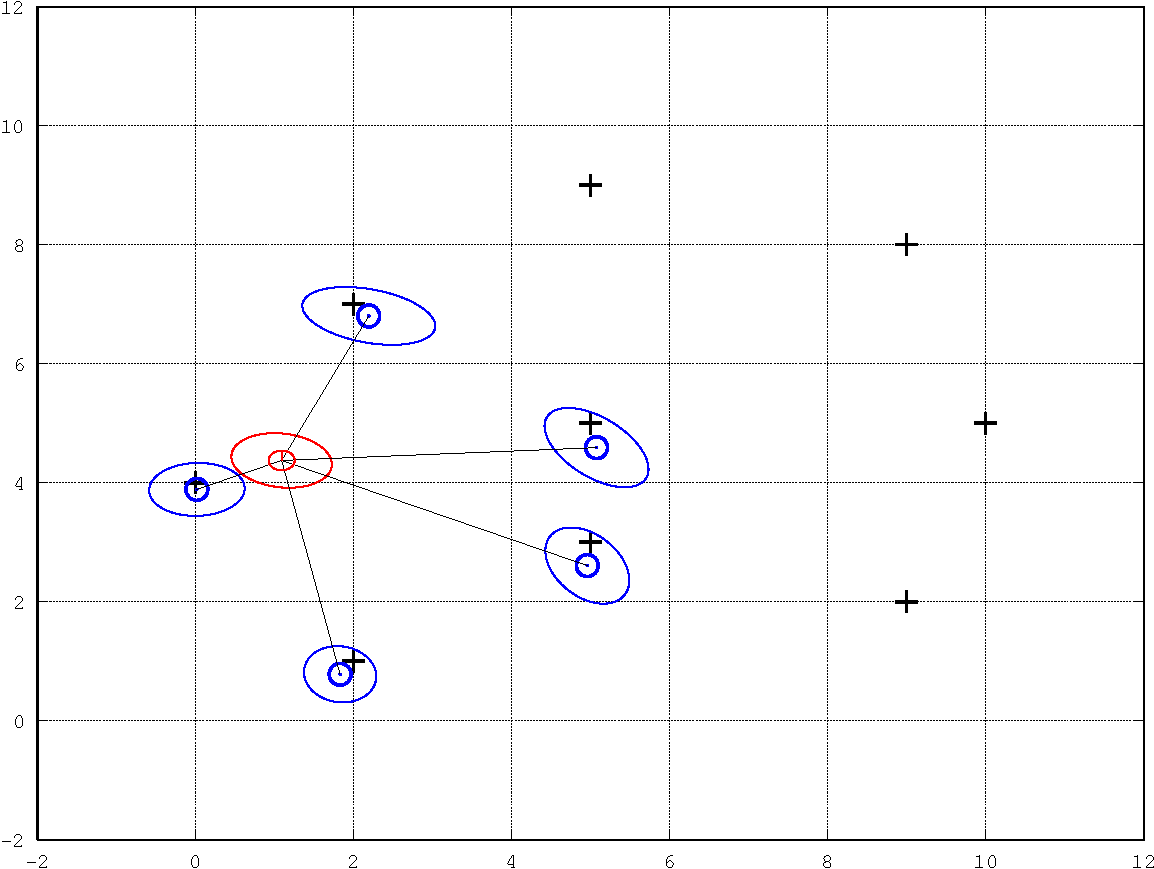
\includegraphics[width=0.32\columnwidth]{ekf_050} &
    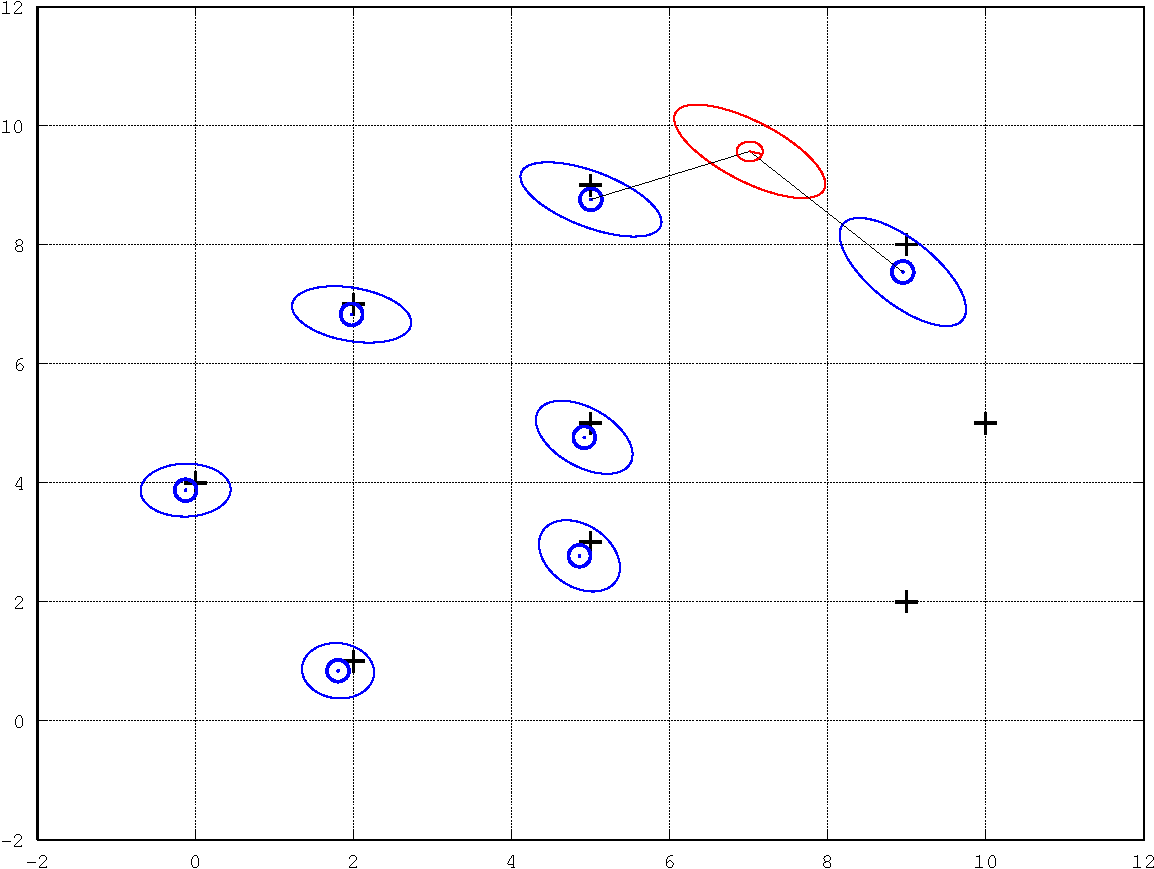
\includegraphics[width=0.32\columnwidth]{ekf_150} &
    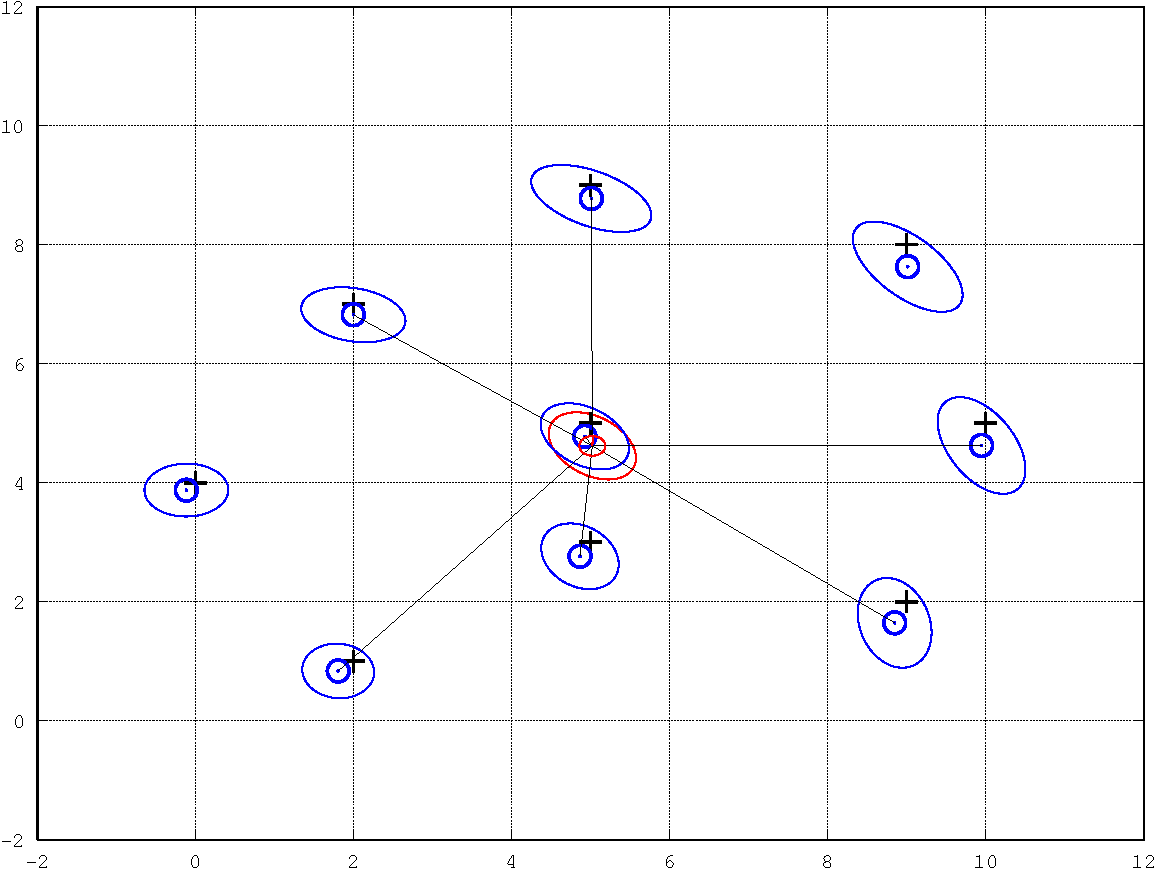
\includegraphics[width=0.32\columnwidth]{ekf_330} \\
    $t=50$ & $t=150$ & $t=330$
  \end{tabular}
  \caption{Example images of the state of the EKF at certain time
  indices.}
  \label{fig:ekfStates}
\end{figure}

%(of size $2N+3 \times 2m$)

Some implementation tips:
\begin{itemize}
    %\item Turn off the visualization to speed up the computation by
        %commenting out the line \texttt{plot\_state(...} in the file
        %\texttt{ekf\_slam.m}.
    \item While debugging, run the filter only for a few steps by
        replacing the for-loop in \texttt{ekf\_slam.m} by
        something along the lines of \texttt{for t = 1:50}.
    \item The command \texttt{repmat} allows you to replicate a given
        matrix in many different ways and is magnitudes faster than
        using for-loops.
    \item When converting implementations containing for-loops into a
        vectorized form it often helps to draw the dimensions of the
        data involved on a sheet of paper.
    \item Many of the functions in \emph{Octave} can handle matrices and
        compute values along the rows or columns of a matrix. Some
        useful functions that support this are \texttt{sum},
        \texttt{sqrt}, and many others.
\end{itemize}

\end{document}
